%%%%%%%%%%%%%%%%%%%%%%% file typeinst.tex %%%%%%%%%%%%%%%%%%%%%%%%%
%
% This is the LaTeX source for the instructions to authors using
% the LaTeX document class 'llncs.cls' for contributions to
% the Lecture Notes in Computer Sciences series.
% http://www.springer.com/lncs       Springer Heidelberg 2006/05/04
%
% It may be used as a template for your own input - copy it
% to a new file with a new name and use it as the basis
% for your article.
%
% NB: the document class 'llncs' has its own and detailed documentation, see
% ftp://ftp.springer.de/data/pubftp/pub/tex/latex/llncs/latex2e/llncsdoc.pdf
%
%%%%%%%%%%%%%%%%%%%%%%%%%%%%%%%%%%%%%%%%%%%%%%%%%%%%%%%%%%%%%%%%%%%


\documentclass[runningheads,a4paper]{llncs}

\usepackage{amssymb}
\setcounter{tocdepth}{3}
\usepackage{graphicx}
\usepackage{epstopdf}
\usepackage{subfig}
\usepackage{array}

\graphicspath{{images/}}

\usepackage{url}
\urldef{\mailsa}\path|ary506@york.ac.uk|
\newcommand{\keywords}[1]{\par\addvspace\baselineskip
\noindent\keywordname\enspace\ignorespaces#1}

\begin{document}

\mainmatter  % start of an individual contribution

% first the title is needed
\title{Gamification of Software Modelling Learning}

% a short form should be given in case it is too long for the running head
\titlerunning{Gamification of Software Modelling Learning}

% the name(s) of the author(s) follow(s) next
%
% NB: Chinese authors should write their first names(s) in front of
% their surnames. This ensures that the names appear correctly in
% the running heads and the author index.
%
\author{Alfa Yohannis}
%
\authorrunning{Gamification of Software Modelling Learning}
% (feature abused for this document to repeat the title also on left hand pages)

% the affiliations are given next; don't give your e-mail address
% unless you accept that it will be published
\institute{Department of Computer Science, University of York, York, United Kingdom\\
\mailsa\\}

%
% NB: a more complex sample for affiliations and the mapping to the
% corresponding authors can be found in the file "llncs.dem"
% (search for the string "\mainmatter" where a contribution starts).
% "llncs.dem" accompanies the document class "llncs.cls".
%

\toctitle{Lecture Notes in Computer Science}
\tocauthor{Gamification of Software Modelling Learning}
\maketitle


\begin{abstract}
Software modelling has a fundamental role in software engineering. However, this subject is relatively perceived difficult for learners require to develop abstraction skill to master the subject. On the other side, gamification has been flourishing as a new popular strategy to engage learners in learning activities. This research attempts to exploit gameful design as an innovative solution to reinforce learners to master software modelling by developing their abstraction skills. Drawing out the gameful design from the Design Lenses and Intrinsic Skill Atoms notions, the pedagogical design from several learning theories and models, as well as being governed by the Design Science Research Methodology and Model-Driven Engineering learning best practices, this research has been developing an early prototype for its software modelling learning gamification. For evaluation, the effects of the artefact are going to be measured using longitudinal controlled experiments.
\keywords{software modelling, gamification, learning, abstraction}
\end{abstract}


\section{Introduction}
Software modelling is commonly perceived as a difficult subject since it requires a lot of abstractions \cite{Borstler2012}. However, this subject has a fundamental and crucial role in software engineering. Failure to master this topic will affect the student’s abstraction capability in analysing and designing a real-world software. Less proficiency in software modelling will likely cause software engineering students facing difficulties completing their degrees, as most of the software engineering related subjects have a sense of intrinsic abstraction problems \cite{Kramer2007}. Their perception of software modelling will affect their attitude towards software engineering today and their career paths in the future.

For new software engineering students, software modelling is commonly perceived as subjects that are difficult to learn. Software, by its nature, is abstract and complex that demand loads of abstraction to model it. This problem is similar to problems in mathematics where much of the concepts can only be accessed through symbolical representations \cite{Duval2006}. Abstraction also means requiring the students to perform information hiding, generalisation, approximation or reformulation, leaving out the irrelevant aspects but keeping the relevant ones, or separation from the concrete reality \cite{Saitta2013}. To overcome these challenges, we need to put more efforts on delivering software modelling in a more concrete and motivating presentation which can engage and ease students to learn it.

On the other hand, the use of games or game elements for serious purposes other than leisure has drawn lots of attention. Gamification \cite{deterding2011game} and Serious Games \cite{Michael2005} have been viewed as solutions to solve motivational problems that emerge when users engage in boring, irrelevant, difficult activities, e.g. Learning sorting algorithms \cite{Yohannis2015} or C-programming \cite{Ibanez2014}.

Therefore, the purpose of this research is to investigate and develop a gamification design framework that systematically and semi-automatically drive gamification design to produce better design software modelling games. More precisely, this research aims to answer the following research questions that are derived from the purpose of this study:
\begin{enumerate}
\item Which processes, aspects, principles, or components of software modelling and their teaching and learning practices that are essential to take into account?
\item What types of game elements and their roles that can deliver software modelling at best? 
\item What kind of framework that orchestrates, design the interaction between, software modelling and game elements to produce a better software modelling gamification?
\item To what extent does gamification of software modelling better engage, motivate, and improve learners’ performances?
\end{enumerate}

\section{Related Works}
Several approaches have been conducted to bring software modelling into a more concrete presentation that can be easily understood by learners, ranging from didactic learning \cite{moisan2009teaching}, modelling tools utilization \cite{Akayama2013}, alternative communication channels and the use of modelling language \cite{Brandsteidl2011}, immersive visual modelling through virtual environment \cite{neubauer2003immersive}, software design studio \cite{Whittle2014}, project-based approach \cite{Szmurlo2007}, to code generation investigation \cite{schmidt2014teaching}. However, most of the approaches have weaknesses in motivating learners to engage continuously, frequently, and actively to learn software modelling, which is the important aspect impacting greatly on learning \cite{Naps2005}. This condition then elevates game as one approach, a.k.a. Game-based learning, to learn or teach software modelling. This method provides students with a new way of learning software modelling, which is not only interactive but also engaging enough to keep them learning continuously. 

The use of game elements for a purpose other than leisure is called gamification \cite{deterding2011game}. Regardless gamification design is still an ongoing challenge \cite{Deterding2013}, it is an opportunity for research that up today there is still no gamification design framework that particularly structures the design of software modelling gamification; a framework that integrates game specific domain into software modelling. Hence, this research aims to develop a gamification design framework of software modelling learning.

Most of the gamification studies available are dominantly related to software engineering in a larger context or other aspects of software engineering, such as software implementation and project management, rather than software modelling in particular \cite{Pedreira2015}. After the literature exploration, only four works have been identified applied gamification for software modelling. They are the works of Groenewegen et al. \cite{Groenewegen2010}, Stikkolorum et al. \cite{Stikkolorum2014}, Richardsen\cite{Richardsen2014}, and Ionita et al. \cite{Ionita2015}. All of the work does not address software modelling learning in general---how learners can learn abstraction in modelling---and they only address very specific topics or area in software modelling, such as activity diagram, coupling and cohesion, and enterprise architectures. Most of the works also only touch the pedagogical aspect superficially or not at all and are validated in a very limited number of respondents. 

\section{Research Methods}
Since the output of this work is designed artefacts, we decided to utilise the Design Science Research Methodology (DSRM) \cite{peffers2007design} as our umbrella methodology. DSRM is selected because it provides a comprehensive high-level conceptual framework how to undergo a full-cycle research process. It also provides six activity guidelines for understanding, developing, executing, and evaluating design artefacts. The six activities are (1) problem identification and motivation activity, (2) defines objectives for a solution activity, (3) set targets for a solution activity, (4) design and development activity, (5) demonstration and evaluation activities, and (6) communication. 

The high-level characteristic means that we can employ other research methods as the sub-methods in each activity. For examples, we employ interviews, literature reviews, and discussion with experts as our methods in problem identification and motivation activity as well as utilise Deterding's lens of intrinsic skill atoms \cite{deterding2015lens} to produce a gameful design in the design and development activity.

\section{Gamfication Design}
To deliver a gameful experience while playing with the artefact, game elements have to be embedded into the artefact's design. Thus, Design Lenses and Skill Atoms \cite{deterding2015lens} are utilised to determine the required game elements as well as the game mechanics. 

\subsection{Design Lenses}
\textbf{Challenge Lens}. The design of the levels has a gradually increased difficulty as well as a variety in its challenges to expose learners to different kinds of domains, models, and diagrams. The onboarding game element is also planned to be implemented into the artefact to help learners familiar with the control system and the flow of the game. The design will also utilise templates to help learners building models without having to start from scratch. The foundation model was already given. They only need to continue the model the meets certain objectives.

\textbf{Goal and Motivation Lens}. The design implements interim goals and intrinsic rewards to motivate learners to engage with the artefact. Every modelling (i.e. object modelling, collaboration modelling) has several stories. A story represents a specific case study to introduce learners to certain problems in specific domains. Every story consists of several levels, and every level has one or more objectives that a student needs to accomplish to complete the level. The level also might be a continuation of its previous level, thus give the learners a sense of step-by-step progression to complete the domain problems. In every story or level, new concepts---related to their type of modelling---or a combination between the old and new concepts might be introduced to learners. Therefore, as the learners progressing, their competence in modelling are being developed--- the intrinsic rewards for the learners. 

\textbf{Action and Object Lens}. A real world problem modelling can be very exhaustive and time-consuming. Thus, the extraneous activities that are not relevant to the core concepts that are being taught should be removed. As a result, learners will be more focused on the main concepts. For that reason, game elements like bite-sized actions (e.g. drag and drop), limited choices (i.e. only limited items can be dragged), and microflow (i.e. put the right element to its right place) are selected to facilitate learners to perform the core activities. Likewise, underdetermination element is also selected to provoke learners' creativity since most of the time there is no single correct model to represent a model; the models can vary. Attractive design is also significant since it draws learners' attention to interact with the artefact.

\textbf{Feedbacks}. The system should give immediate, glanceable, actionable, and graspable to keep learners keep on track and monitor the state of their games. Moreover, the feedbacks should be designed interesting, varied, and appeal to motives to draw their attention, not being boring, and motivating. 

\subsection{Intrinsic Skill Atoms}
The design of the cycle of the game mechanics that the learners will be playing during engaging with the artefact is derived from Intrinsic Skill Atoms, which have six components that should be defined: motivation, goals, actions and objects, challenges, rules, and feedbacks. The main motivation of engaging with the artefact is to master software modelling, which means that they will be able to construct models and solve model-related problems. For an instance, able to build an object modelling of a sign-in screen case. Moreover, The goal of their modelling activities is to meet the given objectives but still in the corridor of the rules. As an example, learners are asked to construct an object diagram of a button that when pressed will clear the text of a textbox. Of course, there will be two objects (button object and textbox object), but the diagram will not be complete if there is no link that connects them to represent their relationship. 

To reach the goals, learners are required to do some actions to manipulate some objects like many other games. The artefact requires learners to perform dragging and dropping and connecting diagram elements (e.g. objects and links) to construct a model as well as the draggable items---contains the names or values of slots, actions, and classes of objects---into the appropriate diagram elements. The learners are confronted with some challenges in the form of problem-solving cases to make the modelling activity more exciting. For an example, an animation that shows how a login page works is displayed to the learners, and they are asked to model it. 

All the models created have to adhere to the rules that are inherent in the types of the models. However, the rules do not always have to be strict with the rules since it could cause the learners demotivated. As an illustration, a link in an object diagram should connect two objects, one on each end. However, this rule can be neglected as long as the rule is not a crucial part of the topic that is being addressed. Finally, feedbacks are required to keep the learners keep track of every action they made, to be informed of their progress, and to motivate them in their ups and downs.

\section{Visual Modelling Editor}
To support developers to design and customise the gamification of software modelling learning---the integration of game elements into its learning activities---at the high level of abstraction and automatically build the generate, this research has been developing the visual modelling editor using Eugenia, a GMF-based graphical model editors \cite{kolovos2015eugenia}. Currently, developers can use the editor to design the gamification of software modelling learning by defining its flows, levels, challenges, and objectives. In the future, this research plans to add more features, such as user-customised types of modelling and diagrams. 

\section{Evaluation}
The controlled experiment will be applied to evaluate the effect of the design artefact. The respondents be divided into two groups, a control group and experimental group. Control will learn software modelling using traditional methods while experimental group will learn with the support from the artefact. After some time learning, they will be given problems to be solved. Their performance will be measured by their ability to solve the problems. To anticipate the order effect, they will be asked to change their roles, from the control group to the experimental group and vice versa. After that, their ability will be tested again using similar problems. After the experiment, the significance of their performance will be calculated. To evaluate the generality of the effects of the artefact, the longitudinal experiment is also considered as well as undergoing the experiment in different countries and universities.

Nonetheless, the controlled experiment is limited only to measure the significance of the design artefact, and no understanding is developed to explain why learning software modelling supported with the artefact is better or worse than the traditional one. Consequently, surveying with questionnaires or interviews might be conducted to investigate the underlying variables or processes. Structural equation modelling also an option if measuring the effects of the identified underlying factors is required. The other alternative method to gain an understanding of underlying variables and processes is through investigating the artefact's event logs using data mining or machine learning techniques.

\section{Conclusion}
In this paper, this research's motivation and problem statements, proposed solution and objectives, research methods, the current progress of the design and development of the artefact, and evaluation plan have been explained. Nevertheless, some interesting aspects of this research have not been covered in this paper due to the limitation of space, such as the architecture of the artefact and the validation methods applied to evaluate models created by learners. So far, this research is focusing its work on software modelling learning. In the future, this research plans to address metamodelling and model transformation learning. 

\subsubsection*{Acknowledgments.} Thanks to our respondents that already participated in our preliminary interview. This research is supported by \emph{Lembaga Pengelola Dana Pendidikan Indonesia} (Indonesia Endowment Fund for Education). 

\bibliography{references} 
\bibliographystyle{ieeetr}

\clearpage
\section{Appendix A: Tables and Images}

\begin{table}[htb]
\caption{Design lenses (game elements) applied in the gamification design.}\label{Table001}
\begin{center}
    \begin{tabular}{ | p{3.2cm} | p {8.7cm} | }
    \hline
	\textbf{Lenses} & \textbf{Elements}\\    
    \hline
    Challenges & Onboarding, scaffolded challenge, varied challenge \\    
    \hline
    Goals and Motivation & interim goals, intrinsic rewards\\
    \hline
	Actions and Object & bite sized actions, limited choices, microflow, underdetermination, sensual \\
    \hline
    Feedbacks & Immediate, juicy, actionable, appeal to motives, glanceable, varied, graspable progress\\
    \hline
    \end{tabular}
\end{center}
\end{table}

\begin{table}[htb]
\caption{Skill Atoms applied in the gamification design.}\label{Table002}
\begin{center}
    \begin{tabular}{ | p{3.2cm} | p {8.7cm} | }
    \hline
	\textbf{Atoms} & \textbf{Description}\\    
    \hline
    Motivation & Master the modelling (solve problem, able to construct model) \\    
    \hline
    Goals & Create models that satisfy requirements \\
    \hline
	Actions and Objects & Construct model using diagrams, elements of a diagram, keywords, hints \\
    \hline
    Challenges & Satisfy requirements, meet objectives\\
    \hline
	Rules & Inherent rules in every model diagram, constraints, objectives\\
	\hline
	Feedbacks & completed objectives, model metrics, and motivating words\\
	\hline
    \end{tabular}
\end{center}
\end{table}

\begin{figure}[htb]
\centering
\subfloat[Level Selection]
	{\frame{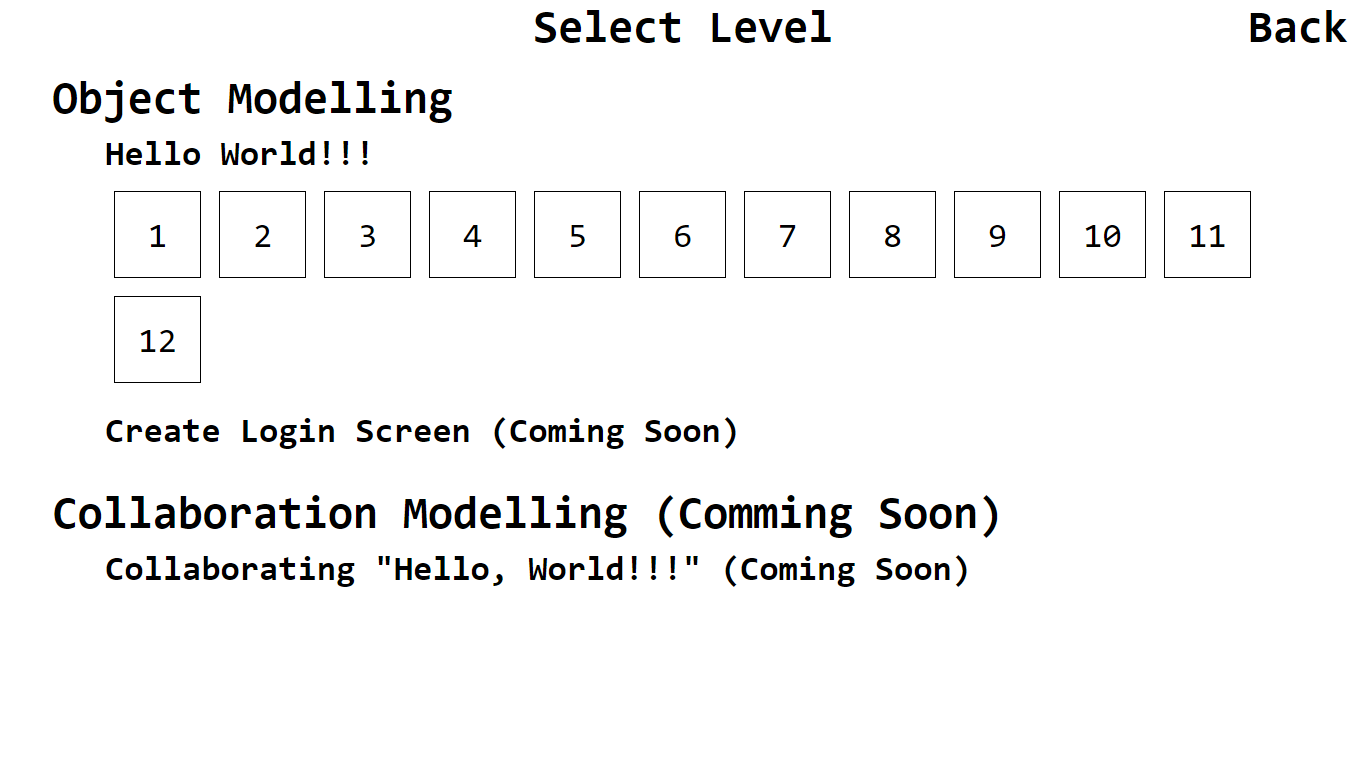
\includegraphics[height=3.5cm]{levels}}\label{Figure001}}
\hspace*{\fill}
\subfloat[Positive Reinforcement]
	{\frame{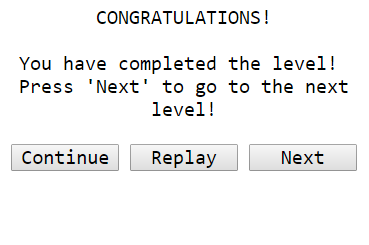
\includegraphics[height=3.5cm]{positive}}\label{Figure002}}
	\caption{Game and learning elements embedded into the artifact.}
\end{figure}

\begin{figure}[htb]
\centering
\frame{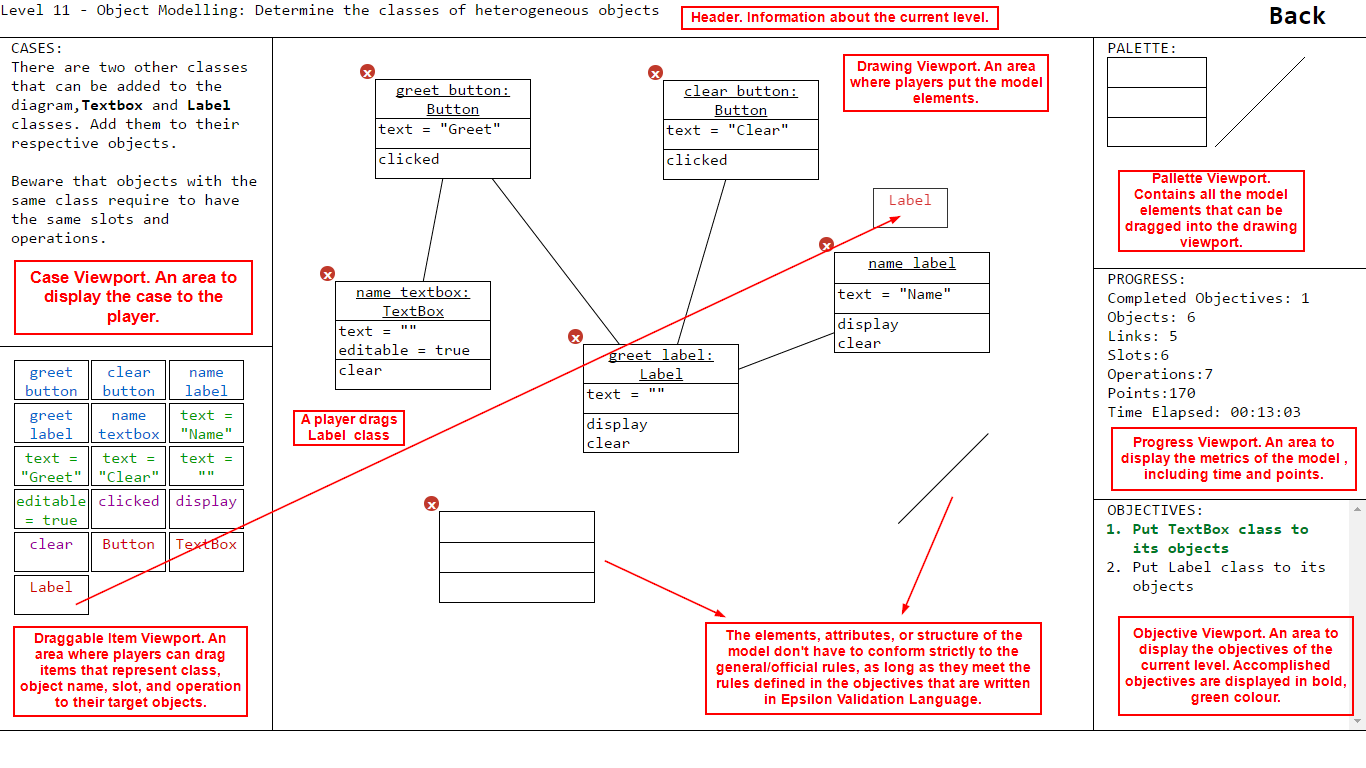
\includegraphics[width=\textwidth]{game-annotated}}
\caption{The game's display.}
\end{figure}

\begin{figure}[htb]
\centering
\frame{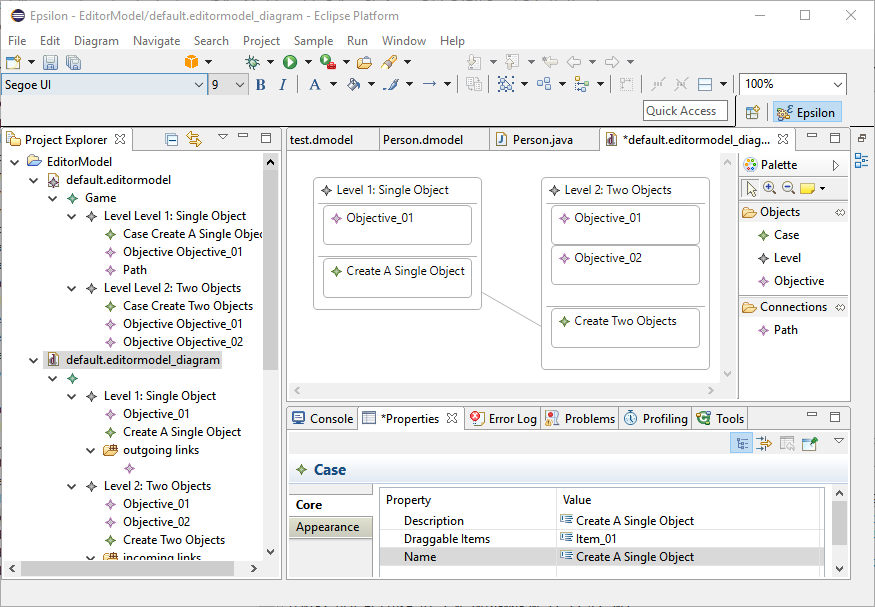
\includegraphics[width=\textwidth]{editor}}
\caption{Game editor to automatically generate the game.}
\end{figure}

\end{document}


